\documentclass[tikz,border=4pt]{standalone}
\usepackage{tikz}
\usetikzlibrary{arrows.meta, positioning, shapes.geometric}

\definecolor{mutblue}{RGB}{30,90,210}

\begin{document}
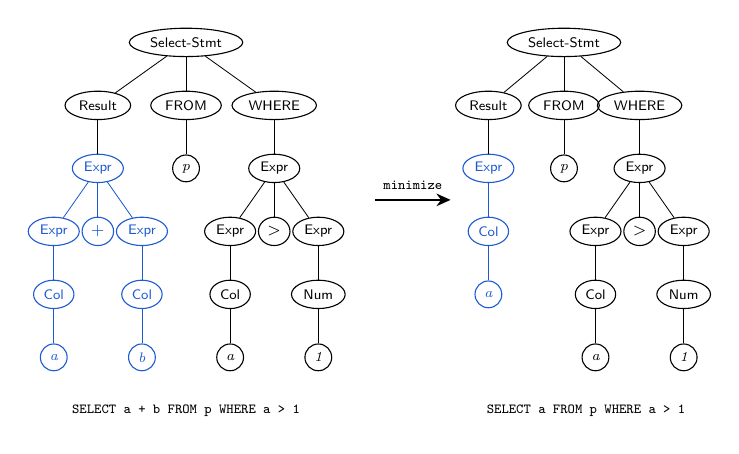
\begin{tikzpicture}[
    x=8mm, y=8mm,
    every node/.style={font=\tiny},
    nt/.style={ellipse, draw=black, line width=0.4pt,
        inner xsep=1.5pt, inner ysep=1pt, font=\tiny\sffamily,
        minimum height=3.6mm},
    op/.style={ellipse, draw=black, line width=0.4pt,
        inner xsep=0.5pt, inner ysep=1pt, font=\tiny\sffamily,
        minimum width=4mm, minimum height=3.6mm},
    lf/.style={circle, draw=black, line width=0.4pt,
        inner sep=0pt, minimum size=3.4mm, font=\tiny\itshape},
    nth/.style={ellipse, draw=mutblue, line width=0.4pt,
        inner xsep=1.5pt, inner ysep=1pt, font=\tiny\sffamily,
        minimum height=3.6mm, text=mutblue},
    oph/.style={ellipse, draw=mutblue, line width=0.4pt,
        inner xsep=0.5pt, inner ysep=1pt, font=\tiny\sffamily,
        minimum width=4mm, minimum height=3.6mm, text=mutblue},
    lfh/.style={circle, draw=mutblue, line width=0.4pt,
        inner sep=0pt, minimum size=3.4mm, font=\tiny\itshape, text=mutblue},
    te/.style={draw=black, line width=0.3pt},
    teh/.style={draw=mutblue, line width=0.3pt},
    mutarrow/.style={-{Stealth[length=1.8mm,width=1.6mm]}, line width=0.6pt},
]

% ====== LEFT: SELECT a + b FROM p WHERE a > 1 ======
\begin{scope}
    \node[nt] (L-root) at (0,0)     {Select-Stmt};

    \node[nt] (L-res)   at (-1.4,-1) {Result};
    \node[nt] (L-from)  at (0,-1)    {FROM};
    \node[nt] (L-where) at (1.4,-1)  {WHERE};

    \node[nth] (L-expr1) at (-1.4,-2) {Expr};
    \node[lf]  (L-p)     at (0,-2)    {p};
    \node[nt]  (L-expr4) at (1.4,-2)  {Expr};

    % Highlighted + expression
    \node[nth] (L-el)   at (-2.1,-3) {Expr};
    \node[oph] (L-plus) at (-1.4,-3) {$+$};
    \node[nth] (L-er)   at (-0.7,-3) {Expr};

    % Comparison
    \node[nt] (L-expr5) at (0.7,-3) {Expr};
    \node[op] (L-gt)    at (1.4,-3) {$>$};
    \node[nt] (L-expr6) at (2.1,-3) {Expr};

    \node[nth] (L-cola) at (-2.1,-4) {Col};
    \node[nth] (L-colb) at (-0.7,-4) {Col};
    \node[nt]  (L-col3) at (0.7,-4)  {Col};
    \node[nt]  (L-num1) at (2.1,-4)  {Num};

    \node[lfh] (L-a1) at (-2.1,-5) {a};
    \node[lfh] (L-b)  at (-0.7,-5) {b};
    \node[lf]  (L-a2) at (0.7,-5)  {a};
    \node[lf]  (L-1)  at (2.1,-5)  {1};

    \foreach \a/\b in {L-root/L-res, L-root/L-from, L-root/L-where,
        L-res/L-expr1, L-from/L-p, L-where/L-expr4,
        L-expr4/L-expr5, L-expr4/L-gt, L-expr4/L-expr6,
        L-expr5/L-col3, L-expr6/L-num1, L-col3/L-a2, L-num1/L-1}
        \draw[te] (\a) -- (\b);
    \foreach \a/\b in {L-expr1/L-el, L-expr1/L-plus, L-expr1/L-er,
        L-el/L-cola, L-er/L-colb, L-cola/L-a1, L-colb/L-b}
        \draw[teh] (\a) -- (\b);

    \node[font=\tiny\ttfamily, anchor=north] at (0,-5.6)
        {SELECT a + b FROM p WHERE a > 1};
\end{scope}

% ====== ARROW ======
\draw[mutarrow] (3.0,-2.5) -- node[above, font=\tiny\ttfamily] {minimize}
                              (4.2,-2.5);

% ====== RIGHT: SELECT a FROM p WHERE a > 1 ======
\begin{scope}[shift={(6,0)}]
    \node[nt] (R-root) at (0,0)    {Select-Stmt};

    \node[nt] (R-res)   at (-1.2,-1) {Result};
    \node[nt] (R-from)  at (0,-1)    {FROM};
    \node[nt] (R-where) at (1.2,-1)  {WHERE};

    \node[nth] (R-expr1) at (-1.2,-2) {Expr};
    \node[lf]  (R-p)     at (0,-2)    {p};
    \node[nt]  (R-expr4) at (1.2,-2)  {Expr};

    \node[nth] (R-col1) at (-1.2,-3) {Col};

    \node[nt] (R-expr5) at (0.5,-3) {Expr};
    \node[op] (R-gt)    at (1.2,-3) {$>$};
    \node[nt] (R-expr6) at (1.9,-3) {Expr};

    \node[lfh] (R-a1)   at (-1.2,-4) {a};
    \node[nt]  (R-col3) at (0.5,-4)  {Col};
    \node[nt]  (R-num1) at (1.9,-4)  {Num};

    \node[lf] (R-a2) at (0.5,-5) {a};
    \node[lf] (R-1)  at (1.9,-5) {1};

    \foreach \a/\b in {R-root/R-res, R-root/R-from, R-root/R-where,
        R-res/R-expr1, R-from/R-p, R-where/R-expr4,
        R-expr4/R-expr5, R-expr4/R-gt, R-expr4/R-expr6,
        R-expr5/R-col3, R-expr6/R-num1, R-col3/R-a2, R-num1/R-1}
        \draw[te] (\a) -- (\b);
    \foreach \a/\b in {R-expr1/R-col1, R-col1/R-a1}
        \draw[teh] (\a) -- (\b);

    \node[font=\tiny\ttfamily, anchor=north] at (0.35,-5.6)
        {SELECT a FROM p WHERE a > 1};
\end{scope}

\end{tikzpicture}
\end{document}